% !TeX program = xelatex
\documentclass[UTF8,zihao=-4,a4paper,fontset=windows]{ctexart}
\usepackage[left=26mm,right=26mm,top=25mm,bottom=25mm]{geometry}
\usepackage{amsmath,amssymb,graphicx,booktabs,array}
\usepackage[hidelinks]{hyperref}
\usepackage{placeins}
\setlength{\emergencystretch}{2em}
\setlength{\parskip}{0.25em}
\raggedbottom
\setlength{\textfloatsep}{14pt plus 3pt minus 3pt}
\renewcommand{\arraystretch}{1.15}
\renewcommand{\topfraction}{0.9}
\renewcommand{\bottomfraction}{0.8}
\renewcommand{\textfraction}{0.08}
\renewcommand{\floatpagefraction}{0.75}
\graphicspath{{../outputs/holdout/figures/}}
\newcommand{\LRFone}{0.7998}
\newcommand{\RFFone}{0.9261}
\newcommand{\CNNFone}{0.5693}
\newcommand{\FusionFone}{0.8526}
\newcommand{\BestName}{随机森林}
\newcommand{\BestFone}{0.9261}
\newcommand{\BestCV}{0.9105}
\newcommand{\BestAccuracy}{0.9213}
\newcommand{\RawRows}{2864056}
\newcommand{\CNNParams}{19052}
\newcommand{\FusionParams}{35868}
\newcommand{\PythonVersion}{3.14.3}
\newcommand{\TorchVersion}{2.12.0+cpu}
\newcommand{\SklearnVersion}{1.9.1}

% 填写真实姓名、班级和学号；不填写虚构身份。
\author{}

\title{多部位时序与统计特征融合的\\人体活动识别研究}
\date{}
\begin{document}
\maketitle
\begin{abstract}
本文基于 PAMAP2 原始数据研究多部位惯性信号的十二类活动识别。手腕、胸部和脚踝的加速度及角速度经过缺失处理、分段和降采样，形成 7410 个离线窗口。以完整连续活动片段为分组单位，将 5187 个窗口用于训练、2223 个用于测试，比例为 7:3；在训练集内进行三折分组交叉验证。比较统计特征逻辑回归、随机森林、早期融合 CNN 及部位时序与统计特征融合模型，测试 Macro-F1 分别为 \LRFone、\RFFone、\CNNFone\ 和 \FusionFone。交叉验证选出的 \BestName\ 取得 \BestAccuracy\ 的测试准确率。单部位和移除部位对照进一步表明，三部位统计特征在本实验中优于各单部位配置，移除手腕带来的性能下降最大。实验保留固定划分、逐折预测和模型回放记录，评价对象为既有受试者的离线活动片段。
\par\noindent\textbf{关键词：}人体活动识别；多传感器融合；分组交叉验证；独立测试；PAMAP2
\end{abstract}
\vspace{0.5em}
\begin{center}\bfseries Human Activity Recognition through Multi-Location Temporal and Statistical Feature Fusion\end{center}
\noindent\textbf{Abstract:} This study compares twelve-class activity recognition on PAMAP2 using wrist, chest and ankle inertial signals. The 7,410 offline windows are split by complete activity segments into 5,187 training and 2,223 test windows (70/30). Three-fold group cross-validation uses only training data and selects the final model before testing. Logistic regression, random forests, an early-fusion CNN and a temporal/statistical fusion network obtain test macro-F1 scores of \LRFone, \RFFone, \CNNFone\ and \FusionFone, respectively. Additional random-forest experiments compare sensor locations. Overlapping windows never cross partitions. The evaluation measures offline activity-segment classification with subject identities shared across training and test sets.
\par\noindent\textbf{Key words:} activity recognition; sensor fusion; group cross-validation; holdout evaluation; PAMAP2
\clearpage

\section{数据描述与研究问题}
可穿戴传感器通过身体不同部位的运动变化描述人体活动。手腕记录局部手臂动作，胸部反映躯干姿态，脚踝提供下肢运动信息。融合这些信号能够同时利用多个部位的观测，但也增加了输入维度和模型训练的复杂度。本文围绕统计特征、时序表示与部位组合展开对比，分析它们在同一数据处理流程下的识别表现。

已有研究使用卷积和循环网络学习可穿戴信号中的活动模式\cite{ordonez,hammerla}。本文设置四种模型：逻辑回归提供统计特征的线性基线，随机森林建模特征间的非线性关系，早期融合 CNN 学习十八通道时序表示，融合模型结合部位编码与统计特征。比较重点是不同表示的识别差异、三部位输入的增益，以及误差集中的活动类别。

相邻窗口存在 50\% 重叠，共享一半采样点。为保持评价数据隔离，本文将同一连续活动片段的全部窗口分配到同一部分，按 7:3 划分训练集和测试集，并在训练集内进行分组交叉验证。这样既保留窗口采样的连续性，也使每个测试片段完整地留在模型拟合之外。

\subsection{数据来源与任务范围}
PAMAP2 由九名受试者佩戴三组惯性测量单元和心率设备采集，完整数据包含十八种活动\cite{uci}。数据分为包含十二种规定活动的 Protocol 和包含额外活动的 Optional。本文仅使用 Protocol，采用手腕、胸部和脚踝的三轴 $\pm16g$ 加速度与三轴角速度，共十八个输入通道。官方说明推荐使用 $\pm16g$ 加速度，以减少较小量程饱和和校准差异的影响\cite{readme}。心率、磁力计、温度、重复量程加速度和无效姿态列不参与本实验。

受试者 109 的 Protocol 记录仅覆盖部分活动，故保留其审计记录但不纳入主实验。主实验采用 101--108 八名受试者，原始共 \RawRows\ 条逐时刻记录。各人的活动覆盖不同，受试者 103 缺少跑步、骑车、北欧式行走和跳绳四类记录。表\ref{tab:data}与图\ref{fig:coverage}给出处理后的覆盖情况。跳绳有 161 个窗口，步行和熨烫各有 921 个窗口，最多类别的样本量约为最少类别的 5.72 倍。该分布是采用类别加权损失和 Macro-F1 的依据。原始文件、压缩包及处理后数组均记录 SHA-256，用于追溯数据版本。

\begin{table}[!htbp]\centering
\caption{主实验数据覆盖与缺失情况}\label{tab:data}
\begin{tabular}{rrrrr}
\toprule
受试者 & 原始记录数 & 活动数 & 窗口数 & 缺失率（\%） \\
\midrule
101 & 376417 & 12 & 956 & 0.291 \\
102 & 447000 & 12 & 1008 & 0.415 \\
103 & 252833 & 8 & 667 & 0.162 \\
104 & 329576 & 10 & 886 & 0.357 \\
105 & 374783 & 12 & 1044 & 0.341 \\
106 & 361817 & 11 & 957 & 0.252 \\
107 & 313599 & 11 & 890 & 0.298 \\
108 & 408031 & 12 & 1002 & 0.442 \\
\bottomrule
\end{tabular}

\par\small 注：缺失率按所选十八个传感器列在该受试者全部原始记录中的缺失元素比例计算；活动数为切窗后有样本的类别数。
\end{table}

\begin{figure}[!htbp]\centering
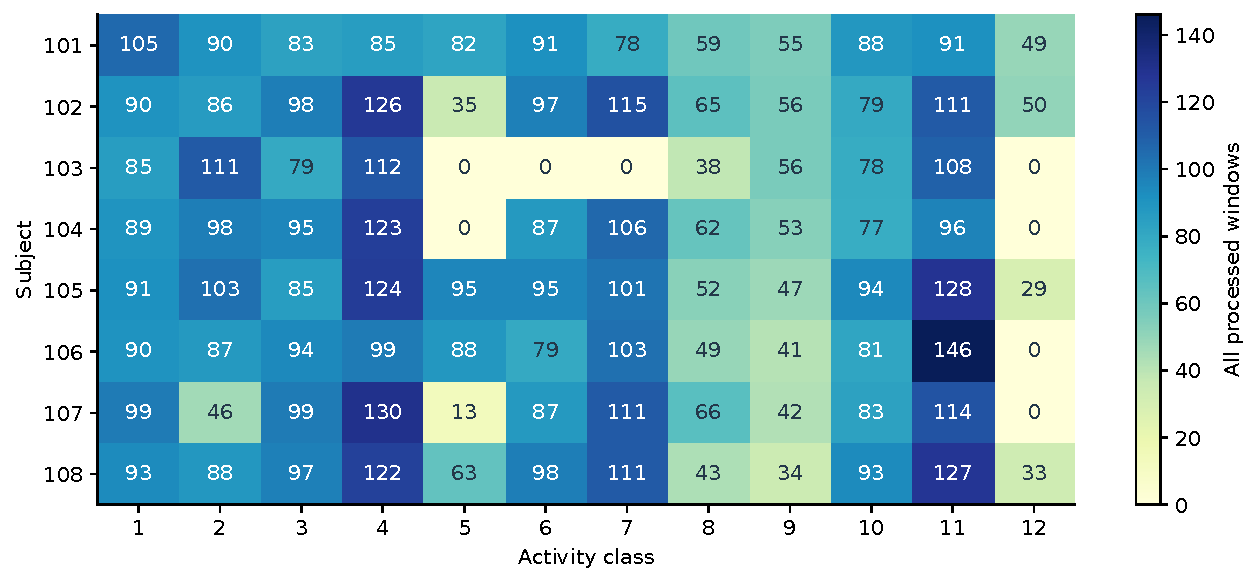
\includegraphics[width=0.94\linewidth]{data_coverage.pdf}
\caption{各受试者与活动类别的窗口数量。零值表示对应活动未产生可用窗口。}\label{fig:coverage}
\end{figure}
\FloatBarrier

\subsection{预处理与窗口构建}
首先按受试者分别处理文件，在活动标签变化、时间戳增量超过 $0.03\,\mathrm{s}$ 或不递增的位置切开记录；不属于规定十二类的过渡标签不保留。任一所选通道若出现超过五十个原始采样点的连续缺失，则排除对应区间并再次切分；不足该阈值的缺失只在当前连续活动段内部插值，段边缘采用最近有效值。插值的作用域因此限定在单个受试者的一段连续活动内。

在原始 $100\,\mathrm{Hz}$ 记录上使用多相低通滤波降采样至 $50\,\mathrm{Hz}$\cite{scipy}，每窗包含 256 点，持续 $5.12\,\mathrm{s}$，步长为 128 点，即相邻窗口重叠 50\%。不足完整窗口的尾部不填充，最终获得 $7410\times18\times256$ 的信号张量。本文将同一连续活动段产生的全部窗口绑定到同一数据部分，因此重叠窗口及同段插值、滤波所使用的信号不会跨越训练与测试。

预处理使用已知活动边界，并在完整片段内利用前后信号完成插值和滤波，评价任务为标注活动内部的离线窗口分类。三部位模型和传感器对照均使用共同可用的窗口，使各配置的差异对应同一批样本上的输入变化。

\section{模型描述}
\subsection{统计特征与标准化}
每个信号通道提取均值、标准差、最小值、最大值、均方根、去均值频谱的谱熵和主频七项特征，六个通道合计四十二维。另对加速度与角速度的三轴模长各提取均值、标准差、最小值和最大值，合计八维。因此每个部位有五十维，三个部位拼接得到 $\boldsymbol f\in\mathbb R^{150}$。设去均值频谱功率为 $P_k$，并将直流项置零，则谱熵为
\begin{equation}
 H=-\sum_k p_k\log(p_k+\epsilon),\qquad p_k=\frac{P_k}{\max(\sum_jP_j,\epsilon)}.
\end{equation}
均值保留各轴的平均信号分量，标准差与均方根描述波动及强度，主频与谱熵描述频谱的集中程度，三轴模长补充整体运动幅度。各项特征均在单个窗口内计算。对于需要标准化的模型，以当前训练部分估计均值和标准差：
\begin{equation}
 z_j=\frac{f_j-\mu_j^{\mathrm{train}}}{\max(\sigma_j^{\mathrm{train}},10^{-6})}.
\end{equation}
神经网络信号输入另按通道在训练窗口和时间轴上估计标准化参数，再将同一变换应用于对应验证集或测试集。统计特征的缩放使不同量纲的变量在逻辑回归正则化和网络优化中采用可比的数值尺度。

\subsection{逻辑回归与随机森林}
逻辑回归使用多类 Softmax 线性分类器，以 L2 正则化限制参数规模，固定 $C=1$、最大迭代数 2000，类别权重采用训练样本的平衡权重。该模型将一百五十维特征映射为十二类概率，作为统计表示的线性基线。

随机森林通过多棵决策树集成建模非线性关系\cite{breiman}。本实验固定 240 棵树、每叶最少两个样本、每次分裂考虑约 $\sqrt d$ 个特征，并采用各自助样本内部的平衡类别权重。不设最大树深度，不进行标准化。单部位和移除部位实验保持树数等设置相同，只改变输入的部位特征列。单部位、双部位和三部位的特征维度分别为 50、100 和 150，分裂候选特征数随 $\sqrt d$ 相应变化。

\subsection{早期融合卷积网络}
早期融合 CNN 将十八通道同时送入卷积编码器。三层卷积的通道数为 $18\to24\to48\to64$，核宽为 $7,5,3$，步长均为 2，每层后接批归一化和 ReLU。时间长度由 256 降至 128、64、32，随后执行全局平均池化、丢弃率 0.25 的 Dropout 和十二类线性分类。该模型参数量为 \CNNParams，不使用人工统计特征。

\subsection{部位时序与统计特征融合}
融合模型为每个部位建立一个独立编码器。每个分支仅接收该部位六通道信号，三层通道数为 $6\to16\to24\to32$，卷积核、步长与早期融合网络一致。每个分支池化后得到三十二维表示。统计特征分支以标准化的一百五十维向量为输入，通过 $150\to64$ 的全连接层、ReLU 和 Dropout，得到六十四维表示。
\begin{align}
 \boldsymbol h_s&=\operatorname{GAP}(E_s(\boldsymbol X_s))\in\mathbb R^{32},\quad s\in\{w,c,a\},\\
 \boldsymbol h_f&=\operatorname{Dropout}(\operatorname{ReLU}(W_f\boldsymbol z+b_f))\in\mathbb R^{64},\\
 \boldsymbol u&=[\boldsymbol h_w;\boldsymbol h_c;\boldsymbol h_a;\boldsymbol h_f]\in\mathbb R^{160}.
\end{align}
最终通过 $160\to64\to12$ 的分类头输出类别。模型参数量为 \FusionParams。三个局部分支分别编码手腕、胸部和脚踝的时间变化，统计分支提供窗口尺度的分布与频谱信息。分类头联合处理这两类表示，使局部时序模式与整体统计量共同参与类别判别。

两个神经网络都使用 AdamW，学习率 $10^{-3}$、权重衰减 $10^{-4}$、批量大小 128，固定训练二十五轮。设当前训练部分第 $c$ 类窗口数为 $n_c$，类别权重采用其平方根倒数，并归一化为均值 1。对一个批次 $\mathcal B$，加权交叉熵为
\begin{equation}
w_c=\frac{n_c^{-1/2}}{\frac1{12}\sum_{j=1}^{12}n_j^{-1/2}},\qquad
\mathcal L=-\frac{\sum_{i\in\mathcal B}w_{y_i}\log p(y_i\mid\boldsymbol X_i,\boldsymbol f_i)}{\sum_{i\in\mathcal B}w_{y_i}}.
\end{equation}
该权重提高稀有类别在损失中的相对贡献，平方根形式使其变化幅度小于计数倒数。每次更新将梯度范数截断为 5。实验使用 CPU、固定随机种子和确定性计算，运行环境为 Python \PythonVersion、PyTorch \TorchVersion、scikit-learn \SklearnVersion。

\section{实验协议与评价指标}
\subsection{固定 7:3 划分与片段隔离}
全部 7410 个窗口按固定留出法分为训练集和测试集：训练集 $N_{\mathrm{train}}=5187$，测试集 $N_{\mathrm{test}}=2223$，满足
\begin{equation}
\frac{N_{\mathrm{train}}}{N_{\mathrm{train}}+N_{\mathrm{test}}}=0.7,\qquad
\frac{N_{\mathrm{test}}}{N_{\mathrm{train}}+N_{\mathrm{test}}}=0.3.
\end{equation}
分组单位为预处理得到的完整连续活动段，共 106 段。每段只对应一个受试者和一种活动，且已在标签变化、时间跳变及长缺失处断开。由于同段窗口重叠且共享插值、滤波上下文，整段必须绑定到同一数据部分。该约束同时用于训练与测试隔离，以及交叉验证各折之间的隔离。

分配程序以活动标签、片段编号和窗口数量为输入，使用混合整数约束分配完整片段\cite{milp}。令 $z_{gr}\in\{0,1\}$ 表示片段 $g$ 是否分到部分 $r$，$r=0$ 为测试集，$r=1,2,3$ 为训练集的三个验证子集，$n_g$ 为该片段窗口数。主要数量约束为
\begin{equation}
\sum_{r=0}^3 z_{gr}=1,\qquad
\sum_gn_gz_{g0}=2223,\qquad
\sum_gn_gz_{gk}=1729\quad(k=1,2,3).
\end{equation}
每部分还要求覆盖十二类活动。在这些约束下，分配程序以减小各类窗口数相对目标比例的偏差为主要目标，求解器在三十秒限时内返回了满足约束的可行划分。整体窗口数精确满足 7:3，类别比例随片段长度变化。例如躺卧活动分为训练 538 个、测试 204 个，上楼活动分为训练 244 个、测试 190 个，具体数量见表\ref{tab:splitclass}。逐窗口清单保存在 \texttt{split\_assignments.csv}，以固定哈希标识，后续训练与复现均使用同一划分。

\begin{table}[!htbp]\centering
\caption{固定数据划分；后三行是训练集内部的三个互斥验证子集}\label{tab:split}
\begin{tabular}{lrrr}
\toprule
数据部分 & 完整片段数 & 窗口数 & 占全部窗口（\%） \\
\midrule
训练集 & 73 & 5187 & 70.00 \\
测试集 & 33 & 2223 & 30.00 \\
训练内第 1 验证折 & 25 & 1729 & 23.33 \\
训练内第 2 验证折 & 23 & 1729 & 23.33 \\
训练内第 3 验证折 & 25 & 1729 & 23.33 \\
\bottomrule
\end{tabular}

\par\small 注：三个验证子集互斥，合计为全部训练集，各占训练集的三分之一。
\end{table}
\begin{table}[!htbp]\centering
\caption{训练、测试与交叉验证各验证折的类别覆盖}\label{tab:splitclass}
\begin{tabular}{lrrrrr}
\toprule
活动 & 训练集 & 测试集 & 验证折 1 & 验证折 2 & 验证折 3 \\
\midrule
躺卧 & 538 & 204 & 181 & 174 & 183 \\
坐 & 495 & 214 & 157 & 174 & 164 \\
站立 & 533 & 197 & 178 & 182 & 173 \\
步行 & 675 & 246 & 256 & 222 & 197 \\
跑步 & 265 & 111 & 88 & 95 & 82 \\
骑车 & 439 & 195 & 170 & 95 & 174 \\
北欧式行走 & 503 & 222 & 115 & 209 & 179 \\
上楼 & 244 & 190 & 95 & 53 & 96 \\
下楼 & 251 & 133 & 91 & 93 & 67 \\
吸尘 & 486 & 187 & 159 & 165 & 162 \\
熨烫 & 647 & 274 & 210 & 218 & 219 \\
跳绳 & 111 & 50 & 29 & 49 & 33 \\
\bottomrule
\end{tabular}

\end{table}

本次评价以完整片段隔离，训练与测试共享受试者身份和采集环境，指标反映既有受试者未参与训练片段的分类表现。同批公开记录已用于前期留一受试者实验；旧协议配置、代码和结果另行留档，本次依据新的固定划分单独统计成绩。

\subsection{仅在训练集内的三折分组交叉验证}
设训练集分为互斥的片段组 $V_1,V_2,V_3$，每组包含 1729 个窗口。第 $k$ 折使用 $T_k=\mathcal D_{\mathrm{train}}\setminus V_k$ 的 3458 个窗口训练，在 $V_k$ 上验证。通过固定折映射实现三折交叉验证\cite{predefined}，每个训练窗口恰好验证一次，2223 个测试窗口不出现在任何一次交叉验证的训练或验证部分。

三折设置由稀有活动的片段数量决定。跳绳共四个完整片段，测试集分配一个含 50 窗口的片段，训练集保留三个片段，分别包含 29、49 和 33 个窗口。每个验证折分配其中一段，使三折均覆盖跳绳和其余十一类活动。所有模型共享这一映射，在相同验证与测试样本上比较。

每次拟合时，逻辑回归的标准化器仅在当前训练折拟合；神经网络的信号、统计特征标准化以及类别权重也只由当前训练折估计。结构、树数、窗口长度及优化参数按配置文件固定，两个网络在各交叉验证折及最终训练中均训练二十五轮。基础种子为 42，三个交叉验证折分别使用 43、44、45，最终训练使用 42。

最终模型的候选集合为逻辑回归、完整三部位随机森林、早期融合 CNN 和融合网络，依据三个验证折固定十二类 Macro-F1 的算术平均值选择。选择记录及各验证成绩哈希先行保存，再将十个预设配置分别在全部 5187 个训练窗口上重新拟合，并在相同 2223 个测试窗口上评价。该流程共包含 $10\times3=30$ 次交叉验证拟合和十次最终拟合，模型选择使用训练阶段记录，最终测试衡量选定配置的留出表现。

\subsection{指标定义与统计范围}
主指标为固定十二类的 Macro-F1：
\begin{equation}
F_{1,c}=\frac{2TP_c}{2TP_c+FP_c+FN_c},\qquad
F_1^{\mathrm{macro}}=\frac1{12}\sum_{c=1}^{12}F_{1,c}.
\end{equation}
同时记录 Accuracy 与宏平均召回率，分母为零时对应类别取零。交叉验证报告三个折的算术平均值与样本标准差：
\begin{equation}
\bar F_{\mathrm{CV}}=\frac13\sum_{k=1}^3F_k,\qquad
s_{\mathrm{CV}}=\sqrt{\frac1{2}\sum_{k=1}^3(F_k-\bar F_{\mathrm{CV}})^2}.
\end{equation}
交叉验证分数用于比较训练阶段表现，测试分数仅由留出测试窗口计算，两者分别报告。三个折的训练数据相互重叠，所报标准差用于描述不同验证片段组合下的成绩波动。

个体测试子集的类别覆盖不同，个体图据其实际出现类别计算 Macro-F1，用于分析误差分布。总体指标则固定十二类并汇总全部测试窗口。两种统计分别描述个体片段的识别质量和完整测试任务的表现。

\section{实验结果与分析}
\subsection{交叉验证与主模型对比}
\begin{table}[!htbp]\centering\small
\caption{训练集内部三折交叉验证的固定十二类 Macro-F1}\label{tab:cv}
\begin{tabular}{lrrrr}
\toprule
模型 & 验证折 1 F1 & 验证折 2 F1 & 验证折 3 F1 & 均值 \\
\midrule
逻辑回归 & 0.9116 & 0.8473 & 0.8901 & 0.8830 \\
随机森林 & 0.9026 & 0.9189 & 0.9101 & 0.9105 \\
仅手腕 & 0.8003 & 0.8301 & 0.8142 & 0.8149 \\
仅胸部 & 0.7699 & 0.8541 & 0.8128 & 0.8123 \\
仅脚踝 & 0.7135 & 0.7708 & 0.7715 & 0.7519 \\
移除手腕 & 0.8386 & 0.8249 & 0.8269 & 0.8301 \\
移除胸部 & 0.8831 & 0.8651 & 0.8723 & 0.8735 \\
移除脚踝 & 0.8705 & 0.9160 & 0.8856 & 0.8907 \\
早期融合 CNN & 0.8147 & 0.7149 & 0.8508 & 0.7935 \\
部位与统计融合 & 0.9310 & 0.8509 & 0.9114 & 0.8978 \\
\bottomrule
\end{tabular}

\end{table}
\begin{table}[!htbp]\centering\small
\caption{主模型的训练交叉验证与固定 30\% 测试集结果}\label{tab:main}
\begin{tabular}{lrrr}
\toprule
模型 & Accuracy & 汇总 Macro-F1 & 个人 F1 均值 $\pm$ SD \\
\midrule
逻辑回归 & 0.8885 & 0.8853 & 0.8807 $\pm$ 0.0744 \\
随机森林 & 0.9236 & 0.9279 & 0.9244 $\pm$ 0.0278 \\
早期融合 CNN & 0.8086 & 0.8132 & 0.8124 $\pm$ 0.1859 \\
部位与统计融合 & 0.9232 & 0.9223 & 0.9195 $\pm$ 0.0298 \\
\bottomrule
\end{tabular}

\par\small 注：F1 均固定十二类；SD 为三个验证折的样本标准差。测试成绩来自同一组 2223 个窗口。
\end{table}
\FloatBarrier
四种主模型中，随机森林的汇总 Macro-F1 最高（0.9279），Accuracy 为 0.9236。融合模型相对随机森林的汇总 F1 差值为 -0.56 个百分点。表\ref{tab:main}同时展示个人均值与离散程度，用于区分总体窗口表现与个体迁移波动。

按个人实际出现类别 F1 进行配对，融合减随机森林的均值为 -0.49 个百分点，受试者重采样百分位区间为 [-2.63, 0.99] 个百分点，探索性符号翻转双侧 $p=0.8750$。这些统计只基于八个配对受试者，不能把区间或单个最好分数当作大样本人群中的保证。

融合与早期 CNN 的输入表示和容量均不同；即使融合成绩较高，也不能只据此证明多分支结构本身有效。现有实验没有单独删除融合模型的统计分支或保持等参数量，因而只能比较完整系统。
\begin{figure}[!htbp]\centering
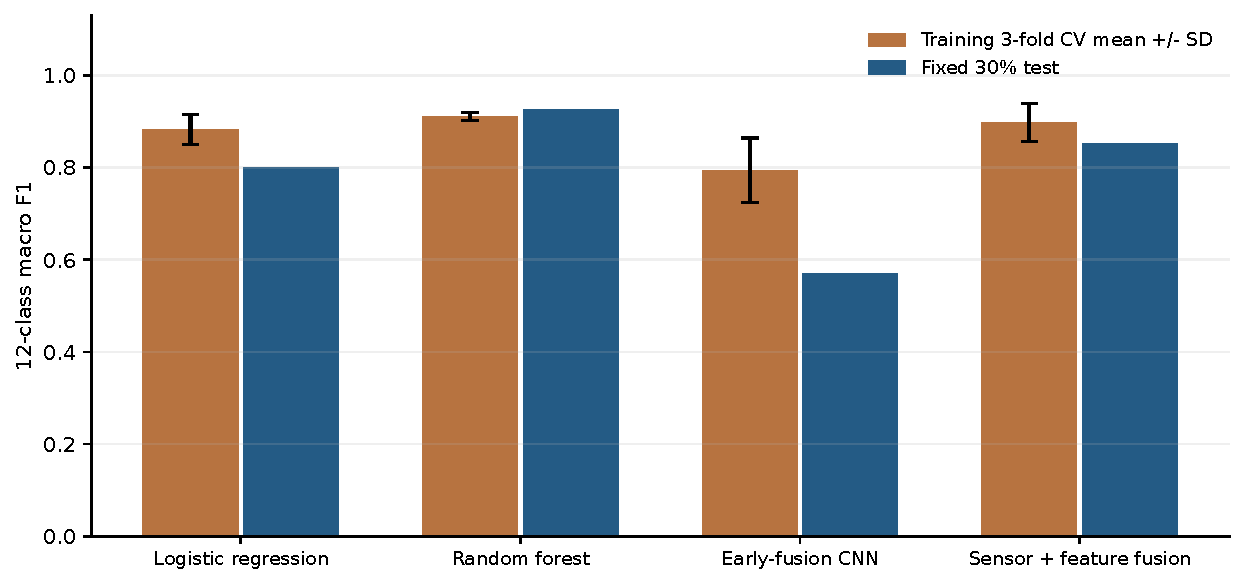
\includegraphics[width=0.96\linewidth]{model_comparison.pdf}
\caption{训练交叉验证均值与最终测试成绩；误差线仅表示验证折间标准差。}\label{fig:models}
\end{figure}
\FloatBarrier

\subsection{传感器部位对比}
\begin{table}[!htbp]\centering\small
\caption{固定随机森林规则下的部位输入对照}\label{tab:ablation}
\begin{tabular}{lrrr}
\toprule
部位输入 & 训练 CV F1 均值 $\pm$ SD & 测试 Accuracy & 测试 F1 \\
\midrule
仅手腕 & 0.8149 $\pm$ 0.0149 & 0.7323 & 0.7497 \\
仅胸部 & 0.8123 $\pm$ 0.0421 & 0.7940 & 0.7690 \\
仅脚踝 & 0.7519 $\pm$ 0.0333 & 0.6946 & 0.7107 \\
移除手腕 & 0.8301 $\pm$ 0.0074 & 0.7962 & 0.8132 \\
移除胸部 & 0.8735 $\pm$ 0.0091 & 0.9118 & 0.9162 \\
移除脚踝 & 0.8907 $\pm$ 0.0232 & 0.8673 & 0.8766 \\
随机森林 & 0.9105 $\pm$ 0.0082 & 0.9213 & 0.9261 \\
\bottomrule
\end{tabular}

\end{table}
\FloatBarrier
单部位实验中，仅胸部的测试 Macro-F1 最高，为 0.7690。完整三部位随机森林为 0.9261；移除实验中移除手腕的测试 F1 最低，为 0.8132。完整配置比最佳单部位高 15.71 个百分点。三组部位对照均使用相同的训练、验证和测试窗口，输入维度分别为 50、100 或 150。

以完整三部位为参照，移除手腕、胸部和脚踝分别降低 11.29、1.00 和 4.95 个百分点。手腕输入在这一特征组合中带来的成绩增量最大。完整配置也高于各双部位配置，说明三个部位的统计表示在本次识别任务中提供了互补信息。
\begin{figure}[!htbp]\centering
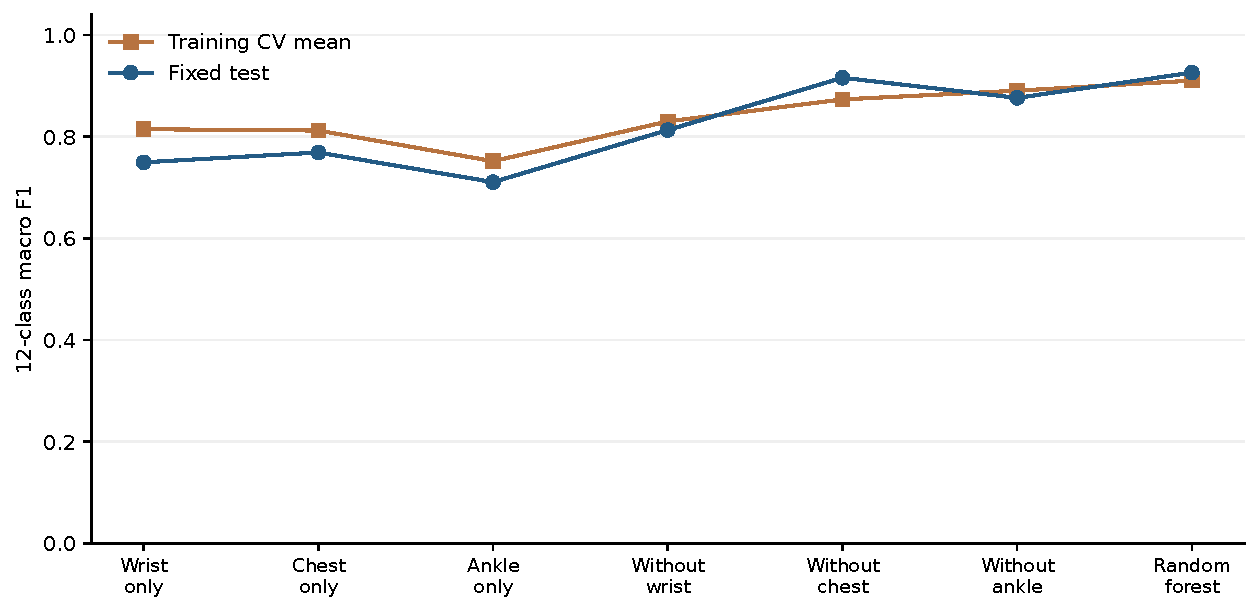
\includegraphics[width=0.96\linewidth]{sensor_ablation.pdf}
\caption{同一划分下的部位实验，分别显示训练交叉验证均值和测试 F1。}\label{fig:ablation}
\end{figure}
\FloatBarrier

\clearpage
\subsection{类别与个体测试片段差异}
融合模型中 F1 较低的三个类别为坐（0.8528）、站立（0.8634）、下楼（0.8817）。与随机森林相比，类别 F1 差值最小的活动为下楼，最大的为北欧式行走。由于各活动的训练覆盖、样本量及动作特征不同，汇总成绩不能替代逐类别分析。混淆矩阵按真实类别逐行归一化，便于查看类别内部的误判分布；它不同于按预测类别归一化的精确率。
\begin{table}[!htbp]\centering\small
\caption{固定测试集的活动窗口数与逐类 F1}\label{tab:class}
\begin{tabular}{rlrrrr}
\toprule
编号 & 活动 & 窗口数 & 逻辑回归 & 随机森林 & 融合模型 \\
\midrule
1 & 躺卧 & 742 & 0.9521 & 0.9655 & 0.9505 \\
2 & 坐 & 709 & 0.8453 & 0.8510 & 0.8528 \\
3 & 站立 & 730 & 0.8290 & 0.8616 & 0.8634 \\
4 & 步行 & 921 & 0.9666 & 0.9629 & 0.9767 \\
5 & 跑步 & 376 & 0.8516 & 0.9714 & 0.9647 \\
6 & 骑车 & 634 & 0.9613 & 0.9710 & 0.9649 \\
7 & 北欧式行走 & 725 & 0.9235 & 0.9562 & 0.9839 \\
8 & 上楼 & 434 & 0.9180 & 0.9310 & 0.9202 \\
9 & 下楼 & 384 & 0.8518 & 0.9314 & 0.8817 \\
10 & 吸尘 & 673 & 0.8079 & 0.8906 & 0.9005 \\
11 & 熨烫 & 921 & 0.8490 & 0.8944 & 0.8956 \\
12 & 跳绳 & 161 & 0.8673 & 0.9477 & 0.9132 \\
\bottomrule
\end{tabular}

\end{table}
\begin{figure}[!htbp]\centering
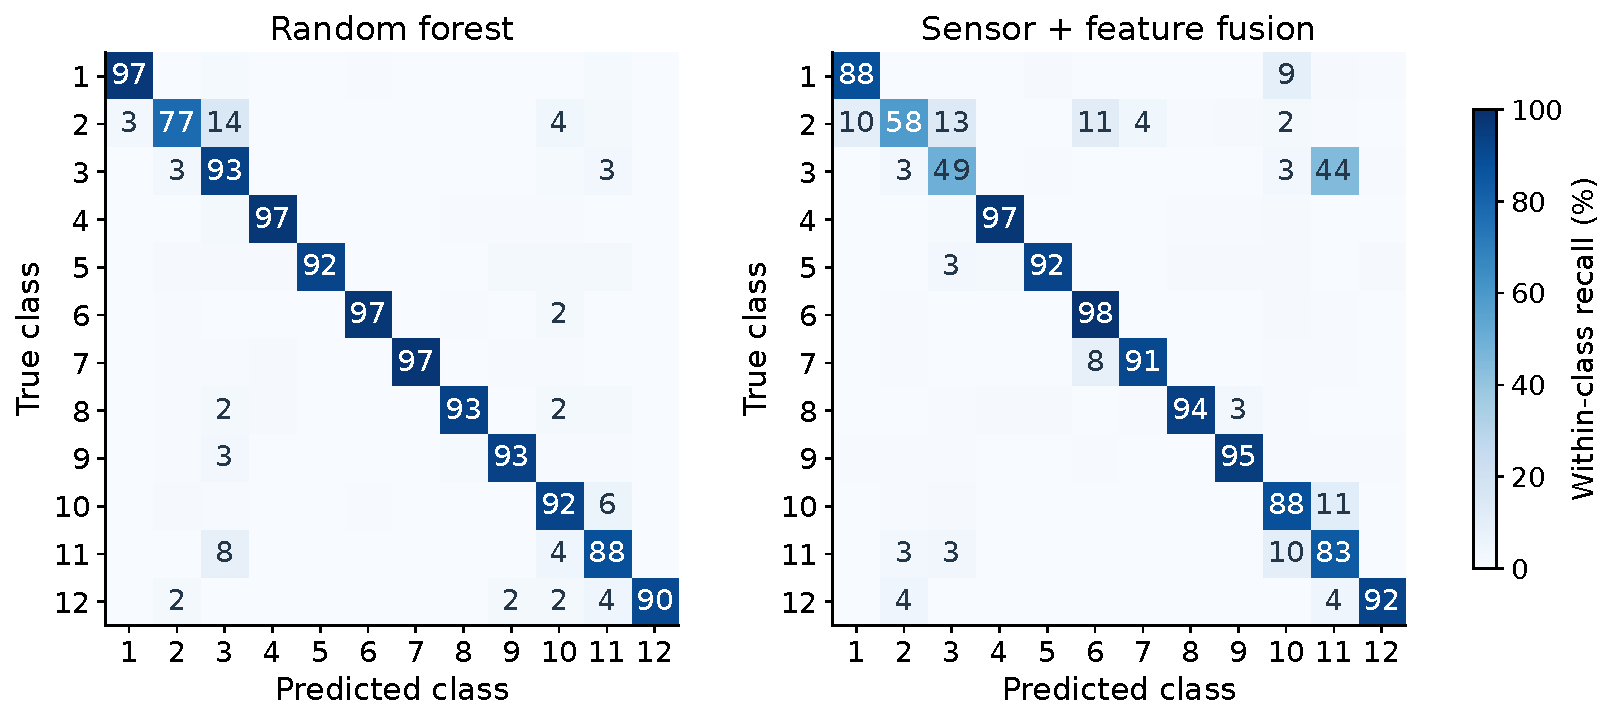
\includegraphics[width=0.98\linewidth]{confusion_matrices.pdf}
\caption{固定测试集的行归一化混淆矩阵，数字为百分比；类别编号对应表\ref{tab:class}。}\label{fig:cm}
\end{figure}
\FloatBarrier
\begin{figure}[!htbp]\centering
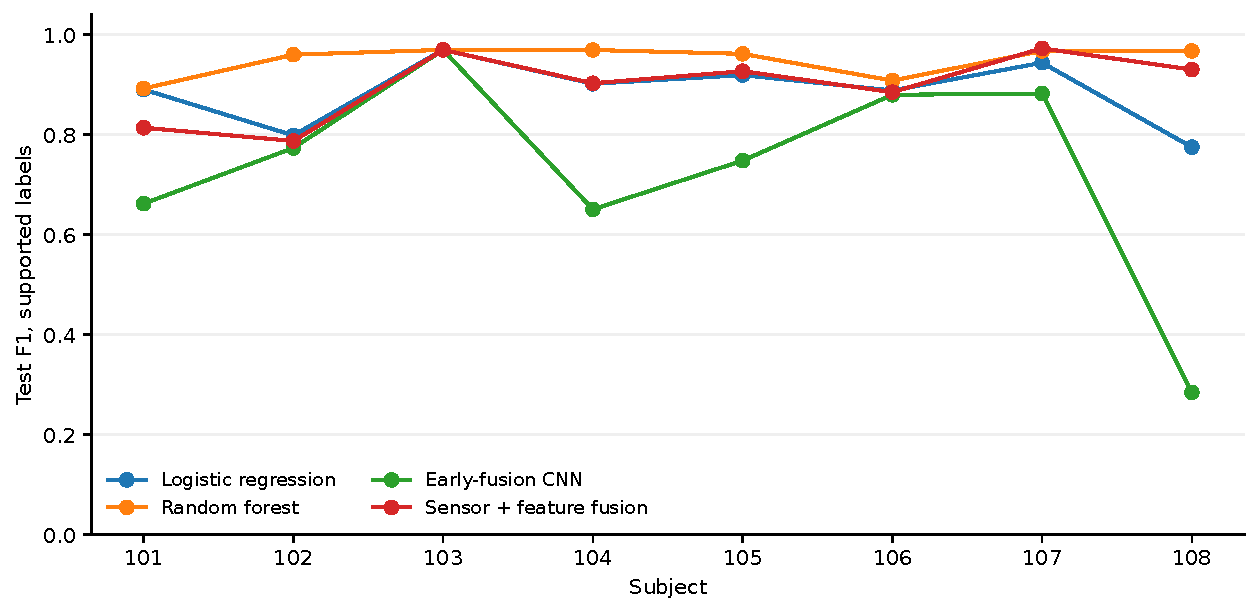
\includegraphics[width=0.96\linewidth]{subject_generalization.pdf}
\caption{各受试者测试子集的 Macro-F1，按该子集实际出现类别计算。}\label{fig:subjects}
\end{figure}
\FloatBarrier
按测试窗口中的实际出现类别计算，融合模型在受试者 102 的测试片段上 F1 最低（0.7875），在受试者 107 上最高（0.9727）。前者包含 313 个窗口、5 类活动，后者包含 411 个窗口、6 类活动。各分数由该测试子集实际包含的类别计算，差异同时反映片段识别表现和活动组合。将个体曲线与逐类混淆结合，可以定位模型在具体人员与活动组合上的薄弱环节。

\subsection{结果核验与模型展示}
分析程序读取四十次拟合保存的窗口索引、真实标签、预测、片段编号和配置哈希，核验样本数量、片段隔离及类别覆盖。检查结果显示，每个训练窗口恰好用于一次交叉验证验证，全部测试窗口保持留出。程序按逐窗口预测重新计算指标，并与训练记录逐项比对；四十个保存模型重新加载后，预测均与原记录一致。论文图表由这些核验结果生成，来源文件和图像以哈希关联。

展示程序加载交叉验证选定的随机森林，其训练数据为 5187 个窗口，与最终测试所评价的模型相同。每个测试类别按窗口索引的 25\% 和 75\% 分位位置各取一个样本，共二十四个窗口，用于演示特征计算、模型加载和类别输出。选样规则在读取预测结果前固定；完整测试集的 2223 个窗口构成正式指标的统计范围。

\section{讨论与结论}
本实验的证据范围由数据和划分方式确定：八名受试者在固定位置佩戴设备，训练与测试以连续活动片段隔离，使用一次 7:3 划分和一个基础随机种子。因此，结果描述这一采集条件下的离线片段分类表现。新增受试者、独立采集会话及多种子重复实验，可进一步量化跨人员、跨会话和初始化带来的变化。

结果呈现出三点规律。第一，统计特征随机森林在交叉验证和最终测试中均居四种主模型首位，说明当前窗口统计量已具有较强的活动区分能力。第二，融合模型的测试 F1 高于早期 CNN，时序编码与统计表示的联合输入在本配置下获得了更好的识别结果。第三，站立、坐和熨烫是融合模型的主要误差来源，类别混淆比总体准确率更直接地指向后续改进目标。

本文完成了从原始传感器记录、缺失处理、窗口构建到模型训练与预测核验的十二类活动识别流程。训练集和测试集按 7:3 固定，模型在训练集内通过三折分组交叉验证选择。最终 \BestName\ 的验证平均 Macro-F1 为 \BestCV，测试 Macro-F1 为 \BestFone，Accuracy 为 \BestAccuracy。三部位特征对照与逐类别预测共同表明，在当前离线片段任务中，完整三部位统计特征随机森林是表现最好的配置。

\clearpage
\begin{thebibliography}{9}
\bibitem{ordonez} ORDÓÑEZ F J, ROGGEN D. Deep convolutional and LSTM recurrent neural networks for multimodal wearable activity recognition[J]. Sensors, 2016, 16(1): 115. DOI: \href{https://doi.org/10.3390/s16010115}{10.3390/s16010115}.
\bibitem{hammerla} HAMMERLA N Y, HALLORAN S, PLOETZ T. Deep, convolutional, and recurrent models for human activity recognition using wearables[EB/OL]. arXiv:1604.08880, 2016. \url{https://arxiv.org/abs/1604.08880}.
\bibitem{uci} REISS A. PAMAP2 Physical Activity Monitoring[DS/OL]. UCI Machine Learning Repository, 2012[2026-10-18]. DOI: \href{https://doi.org/10.24432/C5NW2H}{10.24432/C5NW2H}.
\bibitem{readme} REISS A, STRICKER D. PAMAP2 Dataset: Physical Activity Monitoring, README and data documentation[EB/OL]. 2012[2026-10-18]. \url{https://archive.ics.uci.edu/ml/machine-learning-databases/00231/readme.pdf}.
\bibitem{scipy} SCIPY DEVELOPERS. scipy.signal.resample\_poly[EB/OL]. [2026-10-18]. \url{https://docs.scipy.org/doc/scipy/reference/generated/scipy.signal.resample_poly.html}.
\bibitem{breiman} BREIMAN L. Random forests[J]. Machine Learning, 2001, 45: 5--32. DOI: \href{https://doi.org/10.1023/A:1010933404324}{10.1023/A:1010933404324}.
\bibitem{predefined} SCIKIT-LEARN DEVELOPERS. PredefinedSplit: predefined training and validation folds[EB/OL]. [2026-10-26]. \url{https://scikit-learn.org/stable/modules/generated/sklearn.model_selection.PredefinedSplit.html}.
\bibitem{milp} SCIPY DEVELOPERS. scipy.optimize.milp: mixed-integer linear programming[EB/OL]. [2026-10-26]. \url{https://docs.scipy.org/doc/scipy/reference/generated/scipy.optimize.milp.html}.
\end{thebibliography}
\end{document}
